% !TeX root = ../数模通用模板.tex
\section{问题三的模型建立与求解}
\label{sec:q3}

问题三允许在日内获得新预报并调整购电。本文采用发布时间与提前量匹配的误差校准，将近期误差整日路径输入情景线性规划；按上调加价、下调退回一半费用制定剩余计划，再随实际储电量滚动执行，以平衡提前采购、后续调整和紧急补购的代价。

\subsection{问题三模型的建立}
\subsubsection{输入数据与预测更新}

\textbf{输入与输出。}
输入附件1分时电价、附件2已观察负载与光伏，以及附件3当时发布的未来24小时整点光伏预报。午夜负载采用单HGB、近28日岭校准及前一日偏差半量修正；光伏从0时起即使用当时发布的官方预报，经节点校准和积分后输入调度。输出每日144槽原计划、日内调整后的最终购电量、充放电与储电轨迹，并按指定日期汇总购电费及紧急购电区间。

\textbf{信息集合与剩余时域。}
在每次预报发布时，定义当天剩余时域与可用信息：
\begin{equation}\label{eq:q3-information}
 \mathcal T_\tau=\{r_\tau+1,\ldots,144\},\qquad
 \mathcal I_{d,\tau}=\sigma\!\left(\{L,V\}_{\text{发布前已实现}},
 \{\widetilde V\}_{\text{已发布}},\{p_t\}_{t=1}^{144}\right).
\end{equation}
式中$d$为从0计的日期索引，$t=1,\ldots,144$为日内十分钟槽，槽长$\Delta t=1/6$\,h；$\tau\in\{0,6,12,18\}$为发布小时，$r_\tau=6\tau$为此前已执行槽数。$\mathcal T_\tau$是剩余槽集合，$\mathcal I_{d,\tau}$是可用信息集，$\sigma(\cdot)$表示由括号内数据生成的$\sigma$代数。$L,V$分别为区间平均负载、光伏功率，$\widetilde V$为已发布的整点光伏预报，功率单位均为kW；$p_t$为已知分时电价，单位为元/kWh。

所有预测及购电决策均关于该信息集可测；目标区间实际值只在执行时使用。本次发布的第$h$小时预报记为$\widetilde V_{d,\tau,h}$，其中$h=1,\ldots,24$为发布后的整点序号。

\textbf{光伏节点校准。}
按相同发布小时选取近28日且完整24小时标签已到达的历史预报，残差取
\begin{equation}\label{eq:q3-pv-residual}
 \boldsymbol\epsilon_o=\boldsymbol V_o^{\mathrm{obs}}
 -\mathcal A_o(\widetilde{\boldsymbol V}_o),\qquad
 o+144\le144d+r_\tau,\quad o\in\mathcal H_{d,\tau}.
\end{equation}
式中$o$为历史发布的全局槽号，$\mathcal H_{d,\tau}$为所选历史发布集合。粗体表示向量；$\boldsymbol V_o^{\mathrm{obs}}$为随后144槽的实测平均光伏功率，上标$\mathrm{obs}$表示实测；$\widetilde{\boldsymbol V}_o$为24个官方预报节点。$\mathcal A_o(\cdot)$从该次发布的已观察锚点出发，将节点分段线性积分为144槽平均功率；$\boldsymbol\epsilon_o$为对应残差向量，单位为kW。完整标签条件排除了尚未结束的预报窗口。按14日半衰期形成加权平均误差
\begin{equation}\label{eq:q3-weighted-error}
 \omega_o=2^{-(144d+r_\tau-o)/(14\times144)},\qquad
 \overline{\boldsymbol\epsilon}_{d,\tau}
 =\frac{\sum_{o\in\mathcal H_{d,\tau}}\omega_o\boldsymbol\epsilon_o}
 {\sum_{o\in\mathcal H_{d,\tau}}\omega_o}.
\end{equation}
式中$\omega_o$为历史发布的时间衰减权重，$\overline{\boldsymbol\epsilon}_{d,\tau}$为加权平均残差，$\sum$表示对所列历史发布求和。依据偏差平滑与小样本收缩，求解节点修正量：
\begin{equation}\label{eq:q3-knot-objective}
 \boldsymbol b^{\star}=\arg\min_{\boldsymbol b\in\mathbb R^{24}}
 \left\{\|A\boldsymbol b-\overline{\boldsymbol\epsilon}_{d,\tau}\|_2^2
 +12\|D_2\boldsymbol b\|_2^2+2\|\boldsymbol b\|_2^2\right\}.
\end{equation}
式中$\boldsymbol b$为24个节点的功率修正向量，$\boldsymbol b^\star$为使目标最小的解；$\arg\min$表示取最小值对应的参数，$\mathbb R^{24}$表示24维实向量空间，$\|\cdot\|_2$为欧氏范数。$A\in\mathbb R^{144\times24}$将节点修正映射为区间平均功率修正，$D_2$为二阶差分矩阵。

对式\eqref{eq:q3-knot-objective}求导并令梯度为零，先得到未收缩解，再按历史样本数另作收缩：
\begin{equation}\label{eq:q3-knot-solution}
 \begin{aligned}
 \boldsymbol b^\star_{d,\tau}
 &=(A^{\mathsf T}A+12D_2^{\mathsf T}D_2+2I)^{-1}
 A^{\mathsf T}\overline{\boldsymbol\epsilon}_{d,\tau},\\
 \widehat{\boldsymbol b}_{d,\tau}
 &=\frac{N_{d,\tau}}{N_{d,\tau}+7}\boldsymbol b^\star_{d,\tau},
 \qquad N_{d,\tau}=|\mathcal H_{d,\tau}|.
 \end{aligned}
\end{equation}
式中$\widehat{\boldsymbol b}_{d,\tau}$为收缩后的节点修正量，$N_{d,\tau}$为历史发布数，$|\mathcal H_{d,\tau}|$表示集合的元素个数；$I$为24阶单位矩阵，上标$\mathsf T$和$-1$分别表示矩阵转置与求逆。无可用历史时修正置零。保持官方零发电节点，校准后的节点为
\begin{equation}\label{eq:q3-knots}
 \widehat V^{\mathrm{node}}_{d,\tau,h}
 =\mathbb I(\widetilde V_{d,\tau,h}>0)
 [\widetilde V_{d,\tau,h}+\widehat b_{d,\tau,h}]_+.
\end{equation}
式中$\widehat V^{\mathrm{node}}_{d,\tau,h}$为校准后的节点功率，$\widehat b_{d,\tau,h}$为修正向量的第$h$个分量；$\mathbb I(\cdot)$在条件成立时取1，否则取0；对任意实数$x$，$[x]_+=\max\{x,0\}$表示正部，即取$x$与0中的较大值。

以发布前最后实测功率为第0节点，对各节点作线性插值。由功率与电量的积分关系，未来十分钟区间预测为
\begin{equation}\label{eq:q3-integration}
 \widehat V_{d,r_\tau+i\mid\tau}
 =\frac1{\Delta t}\int_{(i-1)\Delta t}^{i\Delta t}\ell_{d,\tau}(u)\,\mathrm du
 =\frac{\ell_{d,\tau}((i-1)\Delta t)+\ell_{d,\tau}(i\Delta t)}2.
\end{equation}
式中$\ell_{d,\tau}(u)$为节点间的分段线性功率函数，$u$为距发布时刻的小时数，$i=1,\ldots,144-r_\tau$为当天剩余槽的顺序号；$\widehat V_{d,r_\tau+i\mid\tau}$为对应槽的平均光伏功率预测，下标$\mid\tau$标记该预测的发布时刻。每段均位于同一小时线性区间，故梯形积分为精确值；发布时刻的锚点不使用未来实况补齐。

\textbf{负载前缀修正。}
日内取最近至多18个已观察槽的负载预测误差，按6槽半衰期估计偏差：
\begin{equation}\label{eq:q3-load-bias}
 \mu_{d,\tau}=\frac{K_{d,\tau}}{K_{d,\tau}+12}
 \frac{\sum_{j\in\mathcal W_{d,\tau}}2^{-(r_\tau-j)/6}
 (L_{d,j}-\widehat L^0_{d,j})}
 {\sum_{j\in\mathcal W_{d,\tau}}2^{-(r_\tau-j)/6}}.
\end{equation}
式中$\widehat L^0_{d,t}$为当日冻结的HGB午夜负载预测；$\mathcal W_{d,\tau}$为所选已观察槽集合，$K_{d,\tau}$为其槽数，$j$在本式中遍历这些槽。$\mu_{d,\tau}$为估计的负载功率偏差，单位为kW，午夜取$\mu_{d,0}=0$。为减弱短时状态对远期的影响，采用指数衰减更新，并形成净需求电量预测：
\begin{equation}\label{eq:q3-load-net}
 \widehat L_{d,r_\tau+i\mid\tau}
 =[\widehat L^0_{d,r_\tau+i}+\mu_{d,\tau}e^{-(i-1)/36}]_+,
 \qquad
 \widehat n_{d,t\mid\tau}
 =(\widehat L_{d,t\mid\tau}-\widehat V_{d,t\mid\tau})\Delta t.
\end{equation}
式中$\widehat L_{d,t\mid\tau}$为更新后的负载功率预测，单位为kW；$\widehat n_{d,t\mid\tau}$为负载减光伏后的净需求电量预测，单位为kWh；指数项中的$e$为自然常数。

\textbf{同发布时间的相关误差场景。}
对已结束历史日，用其自身在同一发布小时给出的预测构造剩余误差路径：
\begin{equation}\label{eq:q3-path-error}
 \xi_{j,t\mid\tau}
 =\bigl[(L_{j,t}-\widehat L_{j,t\mid\tau})
 -(V_{j,t}-\widehat V_{j,t\mid\tau})\bigr]\Delta t,
 \qquad j<d,\ t\in\mathcal T_\tau.
\end{equation}
式中$\xi_{j,t\mid\tau}$为历史净需求电量误差，单位为kWh；这里$j$为历史日期索引，与式\eqref{eq:q3-load-bias}中遍历槽的局部索引不同。从最近至多28日中按日期等距选取至多7条完整路径，构造情景：
\begin{equation}\label{eq:q3-scenarios}
 n_{s,t\mid\tau}=\widehat n_{d,t\mid\tau}+\kappa\xi_{j_s,t\mid\tau},
 \qquad \sum_{s=1}^{S}\pi_s=1,\quad \kappa=1.
\end{equation}
式中$s=1,\ldots,S$为情景索引，$S$为所选路径数，$j_s$为第$s$条路径的历史日期，$\pi_s=1/S$为等权概率；$n_{s,t\mid\tau}$为情景净需求电量，$\kappa$为误差幅度系数。该构造保留同一天各槽及负载、光伏误差的共同变化。一月不足历史时使用周期冷启动预测，首日无残差路径时采用零偏差情景。

\subsubsection{退款计费与情景线性规划}

\textbf{调整费用。}
按相对午夜原计划的最终净偏差定义调整量：
\begin{equation}\label{eq:q3-adjustment}
 a^+_{d,t}=[q_{d,t}-g^0_{d,t}]_+,\qquad
 a^-_{d,t}=[g^0_{d,t}-q_{d,t}]_+.
\end{equation}
式中$g^0_{d,t}$为午夜锁定原计划，$q_{d,t}$为最后有效版本的常规购电总量，$a^+_{d,t},a^-_{d,t}$分别为最终净上调、净下调量，单位均为kWh；本次发布的购电版本记为$q_{d,t\mid\tau}$。下调取消部分退回原费用的50\%，上调部分另收1.5倍电价，紧急购电按5倍结算。因此实际账单为
\begin{equation}\label{eq:q3-bill}
 C_{\mathrm{tot}}=\sum_{d,t}p_t
 \left(g^0_{d,t}+1.5a^+_{d,t}-0.5a^-_{d,t}+5e_{d,t}\right).
\end{equation}
式中$C_{\mathrm{tot}}$为所统计日期的实际总购电费，单位为元，$e_{d,t}$为实际紧急购电量，单位为kWh；求和覆盖这些日期的全部槽。退款项为负，原计划100\,kWh下调至80\,kWh、$p_t=1$元/kWh时，仅该槽常规购电费为90元。中间被覆盖的未来计划不重复计费，已执行区间冻结；后次调整不受前次计划单调增加的限制。

以下在单日、单次规划中省略日期与发布时刻下标。固定原计划后，常规购电费用连续且分段线性：
\begin{equation}\label{eq:q3-piecewise}
 \phi_t(q_t;g^0_t)=
 \begin{cases}
 0.5p_tg^0_t+0.5p_tq_t,&0\le q_t\le g^0_t,\\
 1.5p_tq_t-0.5p_tg^0_t,&q_t\ge g^0_t.
 \end{cases}
\end{equation}
式中$\phi_t(q_t;g^0_t)$为第$t$槽的常规购电费，单位为元，分号后的$g^0_t$为固定原计划。左右边际成本分别为$0.5p_t$和$1.5p_t$，故不能继续把下调视为被弃余支配的动作。等价线性化为
\begin{equation}\label{eq:q3-adjust-linear}
 q_t=g^0_t+a_t^+-a_t^-,\qquad
 a_t^+\ge0,\quad a_t^-\ge0,\quad q_t\ge0.
\end{equation}
同时增加$a_t^+,a_t^-$会增加$p_t$倍的代价，在正电价下最优解不会利用双向虚假调整获益。

\textbf{逐场景供需与储能约束。}
各场景共享常规购电量，但有各自的储能响应：
\begin{equation}\label{eq:q3-energy}
 q_t+d_{s,t}+e_{s,t}-c_{s,t}-w_{s,t}=n_{s,t},\qquad
 q_t,c_{s,t},d_{s,t},e_{s,t},w_{s,t}\ge0.
\end{equation}
式中$c_{s,t},d_{s,t}$分别为场景充电、放电量，$e_{s,t}$为场景紧急购电量，$w_{s,t}$为场景未利用电量，均为交流侧kWh；$n_{s,t}$为省略发布下标后的场景净需求。由效率关系及跨发布时刻状态继承，有
\begin{equation}\label{eq:q3-soc}
 E_{s,t+1}=E_{s,t}+\eta_c c_{s,t}-d_{s,t}/\eta_d,\quad
 E_{\min}\le E_{s,t}\le E_{\max},\quad
 E_{s,r_\tau+1}=E^{\mathrm{obs}}_{d,r_\tau+1}.
\end{equation}
式中$E_{s,t}$为场景在槽初的内部储电量，$E_{\min},E_{\max}$为其安全下、上界，$E^{\mathrm{obs}}_{d,r_\tau+1}$为本次发布时的实际储电量，单位均为kWh；$\eta_c,\eta_d$分别为单向充电、放电效率。规划中各方向的电量上限为
\begin{equation}\label{eq:q3-power-bound}
 0\le c_{s,t}\le B,\qquad 0\le d_{s,t}\le B.
\end{equation}
式中$B=P_{\max}\Delta t=5000/6$\,kWh为每槽单方向电量上限，$P_{\max}$为单方向最大功率。各情景的储能动作用于估计给定购电量下的短缺代价，最终下发的是共享购电量；真实充放电由当前供需和储电量决定。

\textbf{未来调整机会与目标。}
本次发布后立即执行的六小时只能依靠5倍紧急补购弥补短缺；其后仍有合法更新机会。采用
\begin{equation}\label{eq:q3-opportunity}
 \gamma_{\tau,t}=\begin{cases}
 5,&r_\tau<t\le\min(r_\tau+36,144),\\
 1.5,&r_\tau+36<t\le144
 \end{cases}
\end{equation}
式中$\gamma_{\tau,t}$为场景短缺费用的价格倍数，$\min$取两数中的较小值，将立即执行窗口截于当日日末。该系数近似未来上调机会，18点后全部为5；它只用于规划，真实紧急费始终按式\eqref{eq:q3-bill}计算。该近似未完整表达未来退款和所有后续决策的价值，不作严格多阶段最优性解释。

通过非负辅助变量线性化相邻功率总变差：
\begin{equation}\label{eq:q3-tv}
 v_{s,t}\ge P^{\mathrm{bat}}_{s,t}-P^{\mathrm{bat}}_{s,t-1},\qquad
 v_{s,t}\ge-P^{\mathrm{bat}}_{s,t}+P^{\mathrm{bat}}_{s,t-1},\quad t>r_\tau+1.
\end{equation}
式中$P^{\mathrm{bat}}_{s,t}=(c_{s,t}-d_{s,t})/\Delta t$为场景净充电功率，正值表示充电、负值表示放电；$v_{s,t}\ge0$为相邻槽功率差绝对值的上界，两者单位均为kW。计入购电、短缺、吞吐、功率变化与库存价值后，最终规划为
\begin{equation}\label{eq:q3-objective}
 \begin{aligned}
 \min\quad &\Phi_\tau+\sum_{s=1}^{S}\pi_s\left[
 \sum_{t\in\mathcal T_\tau}\bigl(\gamma_{\tau,t}p_te_{s,t}
 +\lambda_H(c_{s,t}+d_{s,t})\bigr)\right.\\
 &\left.\hspace{2.5em}+\lambda_{\mathrm{TV}}\sum_{t=r_\tau+2}^{144}v_{s,t}
 -\nu_{d,\tau}(E_{s,145}-E_{\min})\right],\\
 \text{s.t.}\quad&\eqref{eq:q3-adjust-linear},\ \eqref{eq:q3-energy}\text{--}\eqref{eq:q3-power-bound},\ \eqref{eq:q3-tv}.
 \end{aligned}
\end{equation}
式中$\Phi_\tau$为本次规划的常规购电目标项。午夜取$\Phi_0=\sum_t p_tq_t$并锁定$g^0_t=q_t$；日内取$\Phi_\tau=\sum_t p_t(1.5a_t^+-0.5a_t^-)$，省略已付且不影响优化的原计划常数。目标前的$\min$表示最小化，$\mathrm{s.t.}$表示满足所列约束；午夜不施加式\eqref{eq:q3-adjust-linear}。

$\lambda_H$为吞吐惩罚权重，取0.005元/kWh；$\lambda_{\mathrm{TV}}$为功率总变差惩罚权重，取0.001元/kW。$\nu_{d,\tau}$为每kWh日末剩余库存的估值系数，$E_{s,145}$为场景日末储电量。

库存估值系数在普通日取$\nu_{d,\tau}=\min_{t\in\mathcal T_\tau}p_t/\eta_c$，评价末日取零。辅助惩罚与终值均不从实际账单抵扣。

式\eqref{eq:q3-objective}为线性规划，各场景分别估计未来储能响应，每次只执行到下一发布时刻，再用新预报和真实储电量重新求解。这样将后续信息更新的作用纳入当前计划，而不直接提前采用尚未发布的信息。单次情景目标的最优解不等同于全年真实费用的全局最优策略。

\subsubsection{实际执行与连续滚动}

当槽实况到达后，根据常规购电与净需求形成的实际余额执行充放电。余额非负时，实际控制为
\begin{equation}\label{eq:q3-feedback-charge}
 \begin{aligned}
 \mathcal B_{d,t}\ge0:\quad
 c_{d,t}&=\mathcal D_{20}\!\left(\min\left\{\mathcal B_{d,t},B,
 \frac{E_{\max}-E_{d,t}}{\eta_c}\right\}\right),\\
 d_{d,t}&=e_{d,t}=0,\qquad w_{d,t}=\mathcal B_{d,t}-c_{d,t}.
 \end{aligned}
\end{equation}
式中$\mathcal B_{d,t}=q_{d,t}+(V_{d,t}-L_{d,t})\Delta t$为交流侧供需余额；$c_{d,t},d_{d,t},e_{d,t},w_{d,t}$分别为实际充电、放电、紧急购电与未利用电量，$E_{d,t}$为实际槽初内部储电量，单位均为kWh。$\mathcal D_{20}(x)=x\mathbb I(x\ge20)$为20\,kWh充电死区算子，$x$为候选充电量，达到阈值才保留，否则取零。

余额为负时，实际控制为
\begin{equation}\label{eq:q3-feedback-discharge}
 \begin{aligned}
 \mathcal B_{d,t}<0:\quad
 d_{d,t}&=\min\{-\mathcal B_{d,t},B,\eta_d(E_{d,t}-E_{\min})\},\\
 c_{d,t}&=w_{d,t}=0,\qquad e_{d,t}=-\mathcal B_{d,t}-d_{d,t}.
 \end{aligned}
\end{equation}
随后按式\eqref{eq:q3-soc}更新真实SOC，只执行到下一次允许更新时间。场景动作不直接平均后下发；日末以
\begin{equation}\label{eq:q3-continuity}
 E_{d+1,1}=E_{d,145},\qquad
 q_{d,t\mid\tau'}=q_{d,t}^{\mathrm{executed}}\quad(t\le r_{\tau'},\ \tau'>\tau)
\end{equation}
式中$E_{d+1,1}$与$E_{d,145}$分别为次日期初和当日日末的实际储电量；$\tau'>\tau$为后续发布时刻，$q_{d,t}^{\mathrm{executed}}$为该槽已执行的常规购电量。由此连续传递状态并冻结前缀，不重置电池电量。

\subsection{问题三模型的求解与结果}

采用HiGHS求解式\eqref{eq:q3-objective}，每次发布的求解时间预算为20\,s。从2025年1月1日6000\,kWh起，使用本节同一规划和反馈规则连续运行365日；一月历史不足时采用前述周期预测和零误差初始路径，随后逐日积累历史，2月接入单HGB基础预测。2月1日实际储电量为1779.6212\,kWh，统计2月1日至12月31日334日、48096槽，末日实际储电量为1200.0000\,kWh。全年1460次线性规划均获得可行解，规划累计耗时125.17\,s，单次最长0.41\,s；本次连续运行与归档耗时127.74\,s。

表\ref{tab:q3-annual}给出评价期账单。原计划费11619999.62元，上调费1043932.12元，下调退款77458.97元，紧急购电费202487.48元，总费用为12788960.26元。最终常规购电量为19832388.1712\,kWh，另有40952.4203\,kWh紧急补购。下调量244156.6289\,kWh表明，退款规则下部分早期购电可在新预报到达后取消。
\begin{table}[H]
\centering\small
\caption{问题三评价期购电费用与运行结果}\label{tab:q3-annual}
\begin{tabular}{lr}
\toprule
指标 & 数值\\
\midrule
原计划费/元 & 11619999.62\\
上调费/元 & 1043932.12\\
下调退款/元 & -77458.97\\
紧急购电费/元 & 202487.48\\
总费用/元 & 12788960.26\\
最终常规购电量/kWh & 19832388.1712\\
下调电量/kWh & 244156.6289\\
紧急购电量/kWh & 40952.4203\\
非空方向反转/次 & 5767\\
\bottomrule
\end{tabular}
\end{table}


\textbf{指定日期结果。}
表\ref{tab:q3-original}、\ref{tab:q3-final}分别列出午夜原计划和最终常规购电量。储能结果两两并排：表\ref{tab:q3-storage-47}与表\ref{tab:q3-storage-140}、表\ref{tab:q3-storage-234}与表\ref{tab:q3-storage-323}分别给出四小时充放电量及起止储电量。紧急购电区间见表\ref{tab:q3-emergency-0}与表\ref{tab:q3-emergency-2}。所有十分钟结果按区间起点展示，四小时结果为该半开区间内24槽电量之和。
\begin{table}[H]
\centering\small
\caption{问题3指定日期的原计划购电量（单位：kWh）}\label{tab:q3-original}
\begin{tabular}{lrrrr}
\toprule
时间段 & 3月20日 & 6月21日 & 9月23日 & 12月21日\\
\midrule
10:00--10:10 & 0.0000 & 0.0000 & 0.0000 & 0.0000\\
12:00--12:10 & 447.5773 & 0.0000 & 294.9785 & 977.8658\\
14:00--14:10 & 0.0000 & 0.0000 & 0.0000 & 0.0000\\
16:00--16:10 & 611.9552 & 96.9398 & 528.3145 & 839.5792\\
18:00--18:10 & 673.7367 & 114.9568 & 742.1825 & 675.9807\\
20:00--20:10 & 0.0000 & 0.0000 & 0.3603 & 0.0000\\
全天电量 & 61349.0929 & 29446.2346 & 64336.0938 & 90241.3602\\
\bottomrule
\end{tabular}
\end{table}
\begin{table}[H]
\centering\small
\caption{问题3指定日期的最终常规购电量（单位：kWh）}\label{tab:q3-final}
\begin{tabular}{lrrrr}
\toprule
时间段 & 3月20日 & 6月21日 & 9月23日 & 12月21日\\
\midrule
10:00--10:10 & 0.0000 & 0.0000 & 0.0000 & 0.0000\\
12:00--12:10 & 500.6572 & 0.0000 & 168.0894 & 942.1100\\
14:00--14:10 & 0.0000 & 0.0000 & 0.0000 & 0.0000\\
16:00--16:10 & 611.9552 & 96.9398 & 528.3145 & 868.0448\\
18:00--18:10 & 706.8097 & 136.8373 & 782.7903 & 675.9807\\
20:00--20:10 & 0.0000 & 0.0000 & 26.3649 & 0.0000\\
全天电量 & 63872.1053 & 30369.8186 & 65296.2037 & 92689.3004\\
全天总费用/元 & 41499.47 & 18009.86 & 42067.72 & 61935.90\\
\bottomrule
\end{tabular}
\end{table}
\begin{table}[H]
\centering\small
\caption{问题3在3月20日的储能结果（单位：kWh）}\label{tab:q3-storage-47}
\begin{tabular}{lrr}
\toprule
时间段 & 充电量 & 放电量\\
\midrule
00:00--04:00 & 7662.8115 & 78.3045\\
04:00--08:00 & 1835.3594 & 6431.5328\\
08:00--12:00 & 2492.6697 & 2677.3195\\
12:00--16:00 & 6300.9854 & 254.7228\\
16:00--20:00 & 555.0210 & 5144.0722\\
20:00--24:00 & 327.9287 & 3105.5341\\
0:00储电量 & \multicolumn{2}{c}{1873.3574}\\
24:00储电量 & \multicolumn{2}{c}{1415.6833}\\
\bottomrule
\end{tabular}
\end{table}
\begin{table}[H]
\centering\small
\caption{问题3在6月21日的储能结果（单位：kWh）}\label{tab:q3-storage-140}
\begin{tabular}{lrr}
\toprule
时间段 & 充电量 & 放电量\\
\midrule
00:00--04:00 & 157.7376 & 878.2834\\
04:00--08:00 & 1094.2404 & 2058.6613\\
08:00--12:00 & 9783.1738 & 0.0000\\
12:00--16:00 & 0.0000 & 0.0000\\
16:00--20:00 & 0.0000 & 6403.8908\\
20:00--24:00 & 1029.2523 & 2748.0573\\
0:00储电量 & \multicolumn{2}{c}{3426.9473}\\
24:00储电量 & \multicolumn{2}{c}{2129.4342}\\
\bottomrule
\end{tabular}
\end{table}
\begin{table}[H]
\centering\small
\caption{问题3在9月23日的储能结果（单位：kWh）}\label{tab:q3-storage-234}
\begin{tabular}{lrr}
\toprule
时间段 & 充电量 & 放电量\\
\midrule
00:00--04:00 & 7701.4622 & 0.0000\\
04:00--08:00 & 1687.1562 & 6537.9082\\
08:00--12:00 & 4906.2508 & 1896.6157\\
12:00--16:00 & 4745.8939 & 444.6634\\
16:00--20:00 & 0.0000 & 5741.0755\\
20:00--24:00 & 1366.7910 & 3355.9961\\
0:00储电量 & \multicolumn{2}{c}{1913.5068}\\
24:00储电量 & \multicolumn{2}{c}{2325.1720}\\
\bottomrule
\end{tabular}
\end{table}
\begin{table}[H]
\centering\small
\caption{问题3在12月21日的储能结果（单位：kWh）}\label{tab:q3-storage-323}
\begin{tabular}{lrr}
\toprule
时间段 & 充电量 & 放电量\\
\midrule
00:00--04:00 & 8621.9853 & 124.9033\\
04:00--08:00 & 3299.7274 & 2580.0109\\
08:00--12:00 & 5042.3042 & 8024.6273\\
12:00--16:00 & 8006.9484 & 2636.9678\\
16:00--20:00 & 0.0000 & 6478.2932\\
20:00--24:00 & 346.2147 & 2758.4698\\
0:00储电量 & \multicolumn{2}{c}{1200.0000}\\
24:00储电量 & \multicolumn{2}{c}{1392.0451}\\
\bottomrule
\end{tabular}
\end{table}
\begin{table}[H]
\centering\small
\caption{问题3指定日期紧急购电区间（单位：kWh）}\label{tab:q3-emergency-0}
\begin{tabular}{lrlr}
\toprule
\multicolumn{2}{c}{3月20日} & \multicolumn{2}{c}{6月21日}\\
时间段 & 电量 & 时间段 & 电量\\
\midrule
09:30--10:00 & 100.0577 & 06:30--07:20 & 176.8897\\
合计 & 100.0577 & 合计 & 176.8897\\
\bottomrule
\end{tabular}
\end{table}
\begin{table}[H]
\centering\small
\caption{问题3指定日期紧急购电区间（单位：kWh）}\label{tab:q3-emergency-2}
\begin{tabular}{lrlr}
\toprule
\multicolumn{2}{c}{9月23日} & \multicolumn{2}{c}{12月21日}\\
时间段 & 电量 & 时间段 & 电量\\
\midrule
20:30--20:40 & 28.2227 & 07:50--08:00 & 4.4020\\
20:50--21:00 & 7.7398 & 10:40--10:50 & 6.8387\\
-- & -- & 20:30--20:50 & 215.7174\\
合计 & 35.9624 & 合计 & 226.9581\\
\bottomrule
\end{tabular}
\end{table}


图\ref{fig:q3-purchase}将四个指定日的原计划与最终量并列，可见调整集中在新预报发布之后，且上调和下调均有发生。图\ref{fig:q3-storage}反映对应储电量随时刻变化的轨迹；同一四小时区间内充电与放电累计量可同时非零，实际十分钟槽内仍只取一个方向。
\begin{figure}[H]
 \centering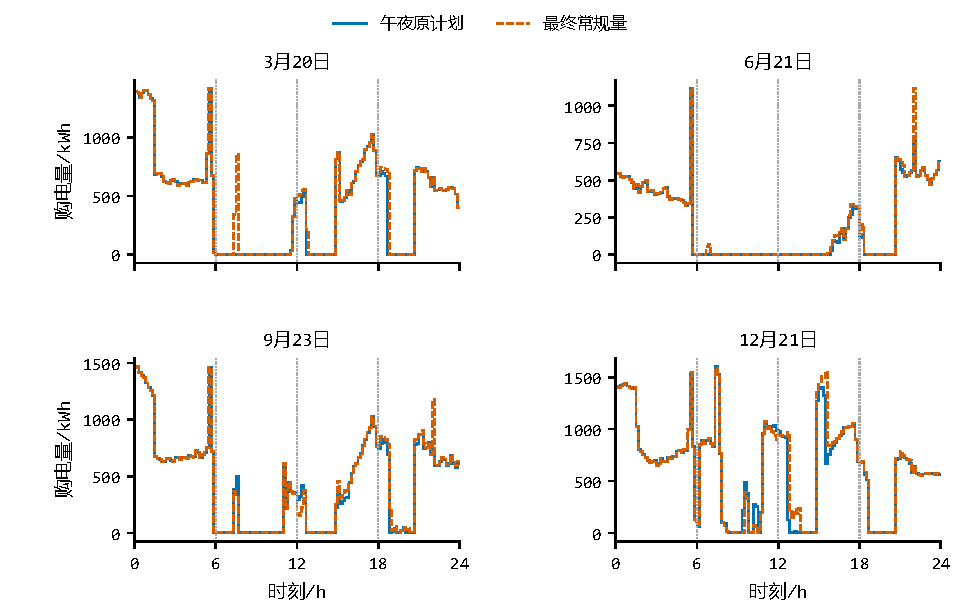
\includegraphics[width=\textwidth]{final_results/q3_purchase.pdf}
 \caption{四个指定日的午夜原计划与最终常规购电量。竖线为6、12、18时的预报发布时间。}
 \label{fig:q3-purchase}
\end{figure}
\begin{figure}[H]
 \centering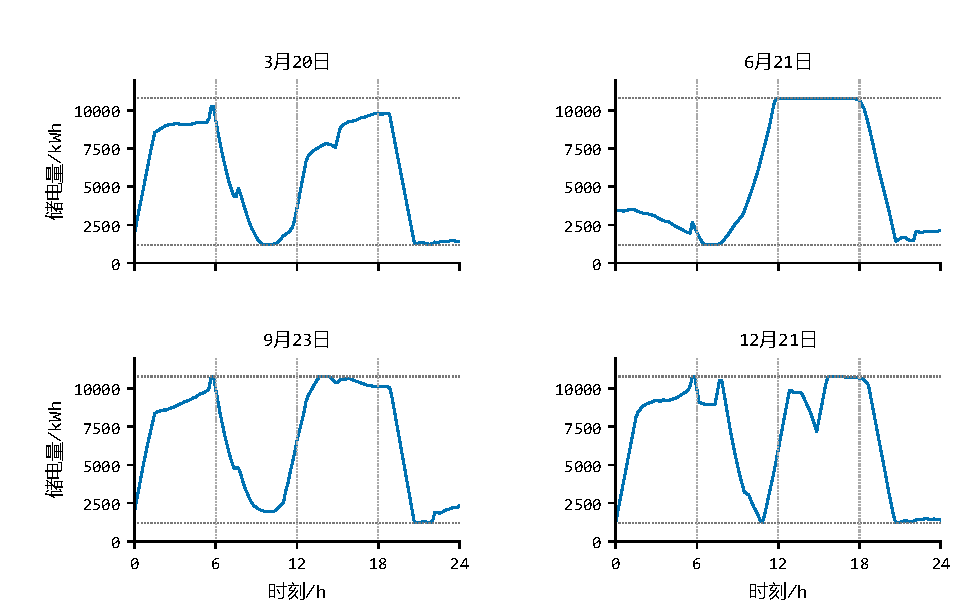
\includegraphics[width=\textwidth]{final_results/q3_storage.pdf}
 \caption{四个指定日的储电量轨迹。左上、右上、左下、右下依次为3月20日、6月21日、9月23日、12月21日；水平虚线为1200与10800\,kWh安全边界。}
 \label{fig:q3-storage}
\end{figure}

图\ref{fig:q3-heat}展示全部评价日的最终调整量，正值表示上调，负值表示下调。各日0至6时已按午夜计划执行，因而该段最终调整量为零；后续调整在各自信息到达后形成。
\begin{figure}[H]
 \centering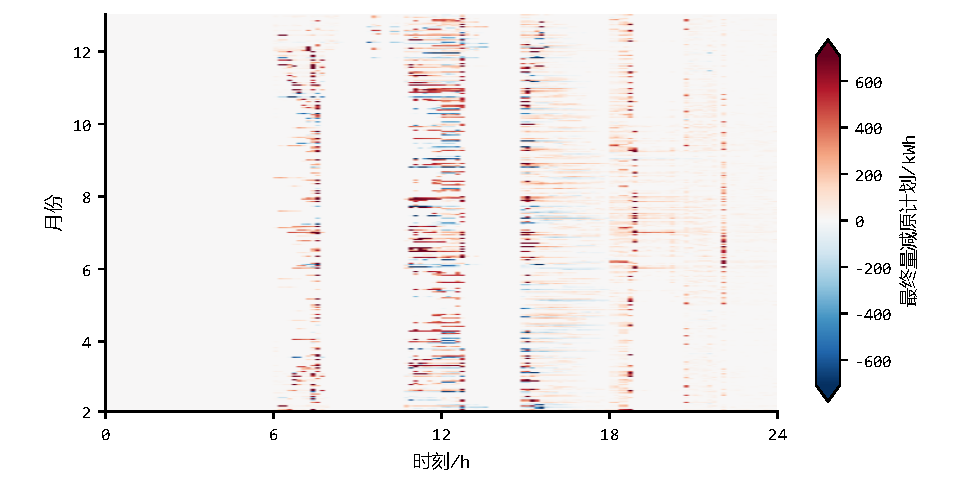
\includegraphics[width=\textwidth]{final_results/q3_adjustments.pdf}
 \caption{2月至12月逐槽最终调整量。颜色表示最终常规量减午夜原计划；色轴在绝对调整量99.5\%分位处截断以显示主要分布，原始值均保留参与费用计算。}
 \label{fig:q3-heat}
\end{figure}

\subsection{模型检验与更新价值分析}

\textbf{预测有效性。}
将各发布后六小时拼接为不重叠评价窗口，并与同一48096槽的午夜预测保持方案比较，见表\ref{tab:q3-prediction}。负载RMSE由192.8553降至184.0852\,kW，光伏RMSE由379.4724降至171.7355\,kW，净需求RMSE由428.9432降至251.8011\,kW。此处午夜光伏已使用0时官方预报，因此比较反映后续预报和负载前缀修正的共同作用。
\begin{table}[H]
\centering\small
\caption{同一48096槽上午夜保持与日内更新的预测误差（单位：kW）}\label{tab:q3-prediction}
\begin{tabular}{lrrrr}
\toprule
变量 & 午夜MAE & 更新MAE & 午夜RMSE & 更新RMSE\\
\midrule
负载 & 144.7736 & 139.6079 & 192.8553 & 184.0852\\
光伏 & 198.8857 & 91.2404 & 379.4724 & 171.7355\\
净需求 & 288.1254 & 187.2121 & 428.9432 & 251.8011\\
\bottomrule
\end{tabular}
\end{table}


\textbf{执行与费用检验。}
对实际轨迹逐槽复算，供需平衡误差为零，SOC递推最大残差小于$10^{-12}$\,kWh，跨日SOC衔接误差为零；储电量与充放电功率均满足题设边界，实际同时充放电和紧急购电用于充电的槽数均为零。四次发布的版本按执行区间拼接后与最终购电量一致，逐槽账单与式\eqref{eq:q3-bill}一致。评价期非空方向反转为5767次，该指标仅计2月至12月内的实际非空方向变化，不把它解释为已标定的电池寿命损失。

\textbf{是否需要其他时刻的预报。}
后续预报降低了实际执行窗口的预测误差，并产生了能够减少早期过量采购的下调动作，因此有理由将6、12、18时预报用于调整。是否每次都必须使用，还取决于调整代价、储能余量和新信息幅度；本次结果没有逐一取消各发布时刻的经济对照，不能据预测精度改善断言每次发布都具有相同的费用收益。完整购电策略保存于\texttt{result3.xlsx}，调整表填写最终总常规电量。
